%{
\documentclass[conference]{IEEEtran}
% IEEE recommendations
\usepackage[cmex10]{amsmath}
\interdisplaylinepenalty=2500
\usepackage{algpseudocode}  % See algorithmicx for documentation.
\usepackage{array}
\usepackage[caption=false,font=footnotesize]{subfig}
\usepackage{stfloats}
\usepackage{url}
\usepackage{float}

% Non-IEEE recommendations:
\usepackage{graphicx}
\usepackage{amssymb}
\usepackage{epstopdf}
\usepackage{multirow}
\usepackage{comment}
\usepackage{arydshln}

% Packages included by VJ, doesn't know if these packages are recommended by IEEE
%\usepackage{color}
\usepackage{cite}
\usepackage{footnote}
%\documentclass[11pt, twoside]{article}   	% use "amsart" instead of "article" for AMSLaTeX format
\usepackage{geometry}                		% See geometry.pdf to learn the layout options. There are lots.
\geometry{letterpaper}                   		% ... or a4paper or a5paper or ... 
%\geometry{landscape}                		% Activate for for rotated page geometry
\usepackage[parfill]{parskip}    		% Activate to begin paragraphs with an empty line rather than an indent
\usepackage{graphicx}				
\usepackage{amssymb}
\usepackage{color}
%\usepackage{matlab-prettifier}
\usepackage{verbatim}
\usepackage{fancyvrb}
\usepackage{multicol}
\usepackage{amsmath}
\usepackage{cite}
\usepackage{bm}
\usepackage{hyperref} 

\sloppy
\definecolor{lightgray}{gray}{0.5}

\title{Reproducing Property of Kernels with XOR, Fibonaaci Spiral and Breast Cancer Datasets}	

\title{Analysis of SVM Kernels in XOR, Double Fibonacci and Real world Datasets}
\author{\IEEEauthorblockN{Gangadharan Esakki}
\IEEEauthorblockA{\{gesakki\}{\tt @unm.edu}\\
               Department of Electrical and Computer Engineering \\
              The University of New Mexico, United States}}
\begin{document}

\maketitle

\section{Introduction} 
\begin{abstract}

In this paper, we introduce the reproducing property of kernels by solving them in Hilbert space for higher dimensional problems.These can be either for linear or non-linear cases where the hyperplane is shattered not just by a single optimal line but rather a complex one. We demonstrate this using the \textit {XOR} problem and \textit {Fibonacci spiral} case. Also in this paper, a real-world dataset from UCI \textit {Breast Cancer Wisconsin} Dataset is studied using SVM kernels and their training and testing errors reported with respect to finding whether a tumor is benign or malignant. 

\end{abstract}

\begin{IEEEkeywords}
HIlbert space, Kernels, XOR, Fibonacci, SVM.
\end{IEEEkeywords}


\section{Kernels: Theory and Background}
Most of the real-world problems are not straight forward and we assume them as linear which is not true in many cases. They are non-linear and have complex relationships between the variables or parameters we take in to solve them. Some algorithms remarkably transform these hard relations to another set of analytic functions and solve them in a different dimension. A mathematically precise core function that effectively does this sort of mapping also called as \textit{Kernel trick} can really change our view to solving and approaching these kind of problems. We can work linear approaches intuitively by passing the data  through non-linear transformation and then work with them non-linearly.If an algorithm is linear, a dual expression can be constructed that expresses the estimator function and parameters as a function of dot products between data. As we know, functions that are dot products in higher dimension Hilbert space. From the \textit{Volterra filter} example,
the transformation of the input space into a polynomial function in Hilbert space solves our problem of estimating the filter in higher space . Equation \ref{eq:volterra} illustrates an order 3 Volterra filter \cite{kernme}


\begin{equation}
\mathbf{z}_n = [1, x[n], x[n-1], x^2[n], x^2[n-1], x[n] x[n-1], x[n]^3, ...]^T
\label{eq:volterra}
\end{equation}

From Equation \ref{eq:volterra} we can then reformulate the problem as Equation \ref{eq:reform} by stating that the function $\hat{y}[n]$ is an approximation of the actual output
given by some parameters multiplied by the input data. The problem, however, with this approach is the \textit{Curse of Dimensionality}.

\begin{equation}
\hat{y}[n] = \mathbf{w}^T\mathbf{z}_n
\label{eq:reform}
\end{equation}

 For a third Voltera filter, we have to pass from a space of 2D dimension, it requries $fact(5, 3) = 10$, but if the input space is in 5D dimensions, then we end up with 56 elements needed which is quite complicated to visualize as our brains are adopted to 3D and cannot go beyond.
 When we increase the number of dimensions, the number of elements begins to explode and is therefore not practical for computation
 for higher order spaces. Hence why we visual creatures come up with this textit{kernel trick} to help solve this problem. The transformation can be generalized by $\mathbf{z}_n = \mathbf{\varphi}(\mathbf{x}_n)$ 
 which in turn allows us to rewrite the estimator function as shown in Equation \ref{eq:rewrite}. 
 
 \begin{equation}
\hat{y}[n] = \mathbf{w}^T\mathbf{\varphi}(\mathbf{x}_n) + b
\label{eq:rewrite}
\end{equation}

To this Equation \ref{eq:rewrite} we choose a function for $\varphi(\cdot)$, the higher dimensional Hilbert space \cite{kernelmethods}. In 
the case of this paper, we have chosen to use the minimum mean square error (MMSE) criterion and a Gaussian Kernel with $\sigma = 1$. From the properties of Hilbert space it is known that functions are dot products in higher dimensions as that's an vital criterion thus verifying the two other properties \textit{Completeness} and \textit{Separability} of the higher space. Every space that satisfies these two properties, will insure that Hilbert Spaces are isometrically isomorphic. To state it more explicitly, a kernel function is one that satisfies Mercer's Theorem \cite{kernelmethods}. The gaussian equation 
used is shown in Equation \ref{eq:gaus_basis}.

\begin{equation}
\mathbf{\varphi(x)} = exp\bigg(\frac{||\mathbf{x} - \mathbf{x}^T||^2}{\sigma^2}\bigg)
\label{eq:gaus_basis}
\end{equation}

the equation of the optimizer is shown here \ref{eq:optimizer} 

\begin{equation}
\mathbf{\alpha} = (\mathbf{\widetilde{K}} + \gamma \mathbf{I})^{-1}\mathbf{y}
\label{eq:optimizer}
\end{equation}

Where $\mathbf{\widetilde{K}} = \mathbf{K} + \mathbf{1}$ and $\mathbf{1}$ is an $N \times N$ matrix of ones. This is a direct result
of building the bias into the Hilbert space $\mathbf{\varphi(\cdot)}$. We can show this in the following steps. 

Let 
\begin{align*}
\mathbf{\widetilde{\varphi}(x)} &= [1, \varphi_1(\mathbf{x}),  \ldots, \varphi_N(\mathbf{x}), \ldots ] \\
\langle\mathbf{\widetilde{\varphi}(x)}, \mathbf{\widetilde{w}} \rangle &= \mathbf{w}^T\mathbf{\varphi(\mathbf{x}}) + b 
\end{align*}

As a result, end up with the following definitions for $\mathbf{\widetilde{w}}$ and $\mathbf{\widetilde{\varphi}}$.
\newcommand{\newPhi}{\mathbf{\widetilde{\varphi}}}

\begin{align*}
 \mathbf{\widetilde{w}} &= 
\begin{bmatrix}
b & \mathbf{w}  \\
\end{bmatrix} \\
\widetilde{\varphi} &= 
\begin{bmatrix} 
\mathbf{1}^T \\
\mathbf{\varphi} \\
\end{bmatrix}
\end{align*}

From here, we simply need to take the inner product of $\mathbf{\widetilde{\varphi}}$ to obtain $\mathbf{K}$. 
\begin{align*}
 \widetilde{\mathbf{K} }&= \langle \newPhi(\mathbf{x}_j), \newPhi(\mathbf{x}_i) \rangle \\
 & = \newPhi^T\newPhi \\
 &= [\mathbf{1}^T, \mathbf{\varphi}] 
 \begin{bmatrix}
 \mathbf{1}^T \\
\mathbf{\varphi} \\
 \end{bmatrix} \\
 &= \mathbf{1}_{N \times N} + \mathbf{\varphi}^T\mathbf{\varphi}
\end{align*}

In order to calculate the bias using the Hilbert space, we first
build the bias into the $\varphi$ variable so that we don't have to treat the equation separately. 

It is also interesting to look at why it is necessary to have $\mathbf{\alpha} = (\mathbf{\widetilde{K}} - \gamma \mathbf{I})^{-1} \mathbf{y}$ 
instead of $\mathbf{\widetilde{K}}^{-1}\mathbf{y}$. The reason for this is that we cannot guarantee that $\mathbf{\widetilde{K}}$ is well posed and pre-conditioned.
For example, the gamma value multiplied by the Identity matrix (I) makes sure that we have enough data points than dimension, otherwise it would lead to more noise in the data generation process. This also leads to another problem of overfitting the data and we need to add penalty term or a regularizer. Usually we can add L1 norm regularization also called as LASSO or else we can go for \emph{L2 norm regualarization} also known as \emph{Ridge Regression}. This is expressed by means of a regularizer, an extra term which controls the estimator function boundaries and avoid over-fitting by minimizing the coefficients of the solution with slight adjustment of parameter c. In the case of ridge regression this allows you to choose better fit or lower coefficients.
The \emph{ridge regression} corresponds to solving the following equation: 

\begin{align*}
\underset{\mathbf{w}}{\text{min}} \mathbf{\mathcal{L}}_\lambda (\mathbf{w}, S) &= 
\underset{\mathbf{w}}{\text{min}} \lambda ||\mathbf{w}||^2 + \sum_{i=1}^{l}(y_i - g(\mathbf{x}_i))^2
\end{align*}

Here, $\lambda$ represents the relative trade-off between the L2 norm and the loss \cite{kernelmethods}. In order to find the minimum of this equation, 
we need to take the derivative as shown below: 

\begin{align*}
\mathbf{X}^T\mathbf{X}\mathbf{w} + \lambda\mathbf{w} = (\mathbf{X}^T\mathbf{X} + \lambda \mathbf{I}_n)\mathbf{w} = \mathbf{X}^T\mathbf{y}
\end{align*}

Here, $\mathbf{X}$ is just the input space where each row is $\mathbf{x}_1, \ldots, \mathbf{x}_N$. Here in this problem  the input space into an infinite dimensional Hilbert space show below: 

\begin{align*}
\mathbf{\Phi}^T\mathbf{\Phi}\mathbf{w} + \lambda\mathbf{w} = (\mathbf{\Phi}^T\mathbf{\Phi} + \lambda \mathbf{I}_n)\mathbf{w} = \mathbf{\Phi}^T\mathbf{y}
\end{align*}

These equations can be solved by, $\mathbf{w}$: 
\begin{align*}
\mathbf{w} = \lambda^{-1} \mathbf{\Phi}^T (\mathbf{y} - \mathbf{\Phi} \mathbf{w}) = \mathbf{\Phi}\mathbf{\alpha}
\end{align*}

This is possible because we know that $\mathbf{w}$ can be written as a linear combination of the input space. And then finally we can solve
for $\mathbf{\alpha}$.

\begin{align*}
\bm{\alpha} = \lambda^{-1}(\mathbf{y} - \mathbf{\Phi} \mathbf{w}) \\
\mathbf{y} = (\mathbf{\Phi \Phi}^T + \lambda\mathbf{I}_N)\mathbf{\alpha}
\end{align*}

From here we can see that all we have to do is a substitution from our original equation in \ref{eq:optimizer} to see that
$\lambda\bm{I}_N$ is just $\gamma\bm{I}_N$ which is used as a regularization parameter and controls the coefficient vectors which in turn minimize the complexity 
of the system. 

\section{SVM Kernels: Methodology and Experiments}
In this section, we will deal about how SVM experiments with XOR Toy problem and Double Fibonacci spiral. Additionally, the Breast Cancer dataset from UCI is also studied to learn more about kernels and how they analyze the real-world dataset. In the first part of this section, we want to look at how well the SVM works using
100 data points for training, and then 1000 points for testing. We will
then validate the methods using \textit{MATLABS}'s v-fold function. The
second part is to then investigate the Double Fibonacci spiral applying
the same techniques as mentioned above. For the \textbf{Breast Cancer UCI dataset}, I applied k-fold cross validation and sampled the training and testing datasets with \textit{R Studio}, the standard language for Statistics and used in Data Analysis. I have given all the results for the three experiments and analyzed them accordingly.

\subsection{XOR problem}
We begin this section by first illustrating the \textit{XOR} problem. In figure 
\ref{fig:XOR} \& \ref{fig:MMSE}, we have labeled 4 set of points with one class in red, and the other class in blue constructed using Gaussian kernel and MMSE criterion. From this figure, we can see that there is no obvious way to separate the data in 2D dimensional space. So now we are going to pass it to Hilbert space based on the training set of points and solve them in higher dimension with unseen testing data points to generate the XOR function and see how the dual parameter $\alpha$s varies.  

\begin{figure}[ht!]
\centering
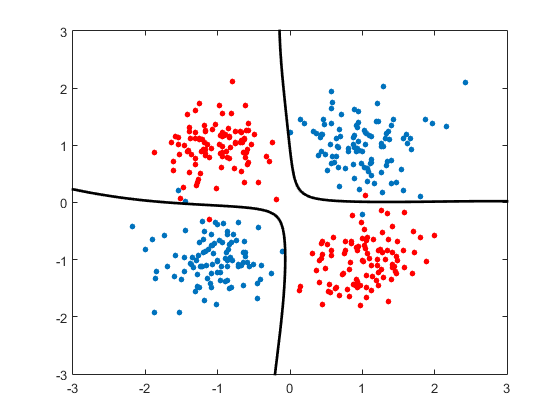
\includegraphics[width=0.5\textwidth]{figs/XOR.png}
\caption{XOR Toy Data}
\label{fig:XOR} 
\end{figure}

\begin{figure}[ht!]
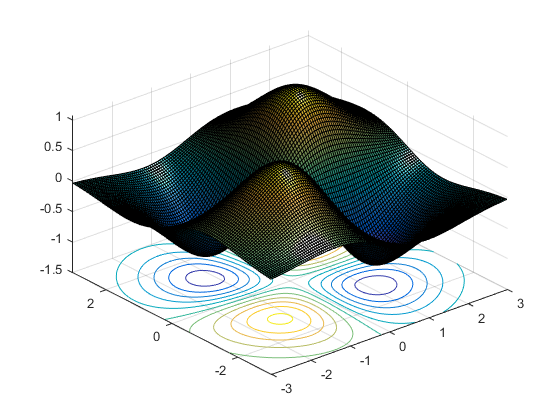
\includegraphics[width=0.5\textwidth]{figs/MMSE.png}
\caption{MMSE}
\label{fig:MMSE} 
\end{figure}

This testing phase of 1000 points based on the SVM kernel we trained is for a special case here. With the hyperplane separating the blue and red points to  
we can take the values that we have generated and plot them in 3D space and then project the hyperplane with the plane $ z=0$. This is illustrated
in Figure \ref{fig:SVM_XOR_HYP}.

\begin{figure}[ht!]
\centering
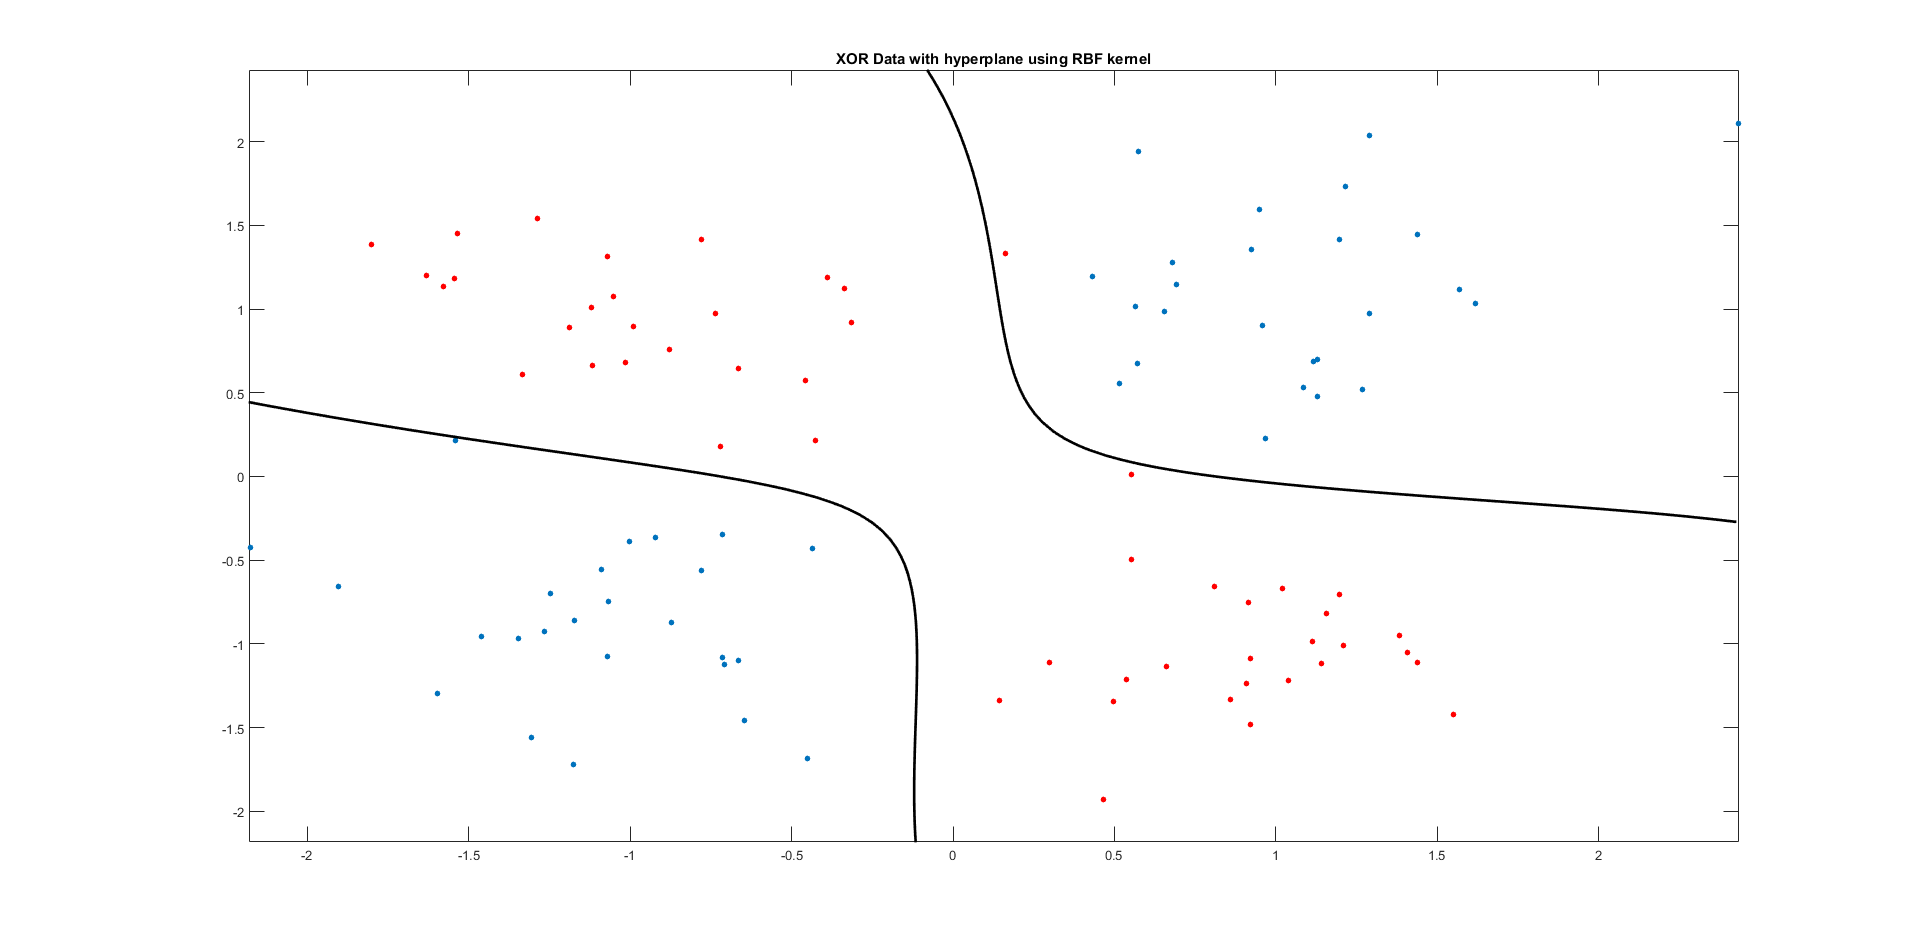
\includegraphics[width=0.5\textwidth]{figs/SVM_XOR_HYP.png}
\caption{SVM XOR Data Hyperplane separation using a radial basis function}
\label{fig:SVM_XOR_HYP} 
\end{figure}

With the test points we cross validated to test its performance. To do this, we pass the training model to saved dual parameter $\bm{\alpha}$ which we calculated in the training phase. The output from the k-fold(k=5) cross-validation of this operation the classifier is working very well with a classification rate of nearly 96\%. 


\subsection{Fibonacci Spiral Problem}
The Double Fibonacci spiral \ref{fig:fibo_spiral} is a nice example of non-linear classification and with RBF kernels it would make a special case study of how the hyperplane is going to be projected with such complex datasets.

\begin{figure}[h!]
  \centering
  	\caption{Fibonacci Spiral with
		(a) Double Spiral Fibonacci with 1000 points. 
	    (b) Contour plot with hyperplane projected in 3D
	    (c) Hyperplane projected in 2D with separation.  
    }
  	\subfloat[Double Fibonacci Spiral]
		{
\includegraphics[width=0.242\textwidth]{figs/FB_spiral_WHYP.png}
  				\label{fig:fibo_spiral}} 
	\subfloat[Contour plot]
  	{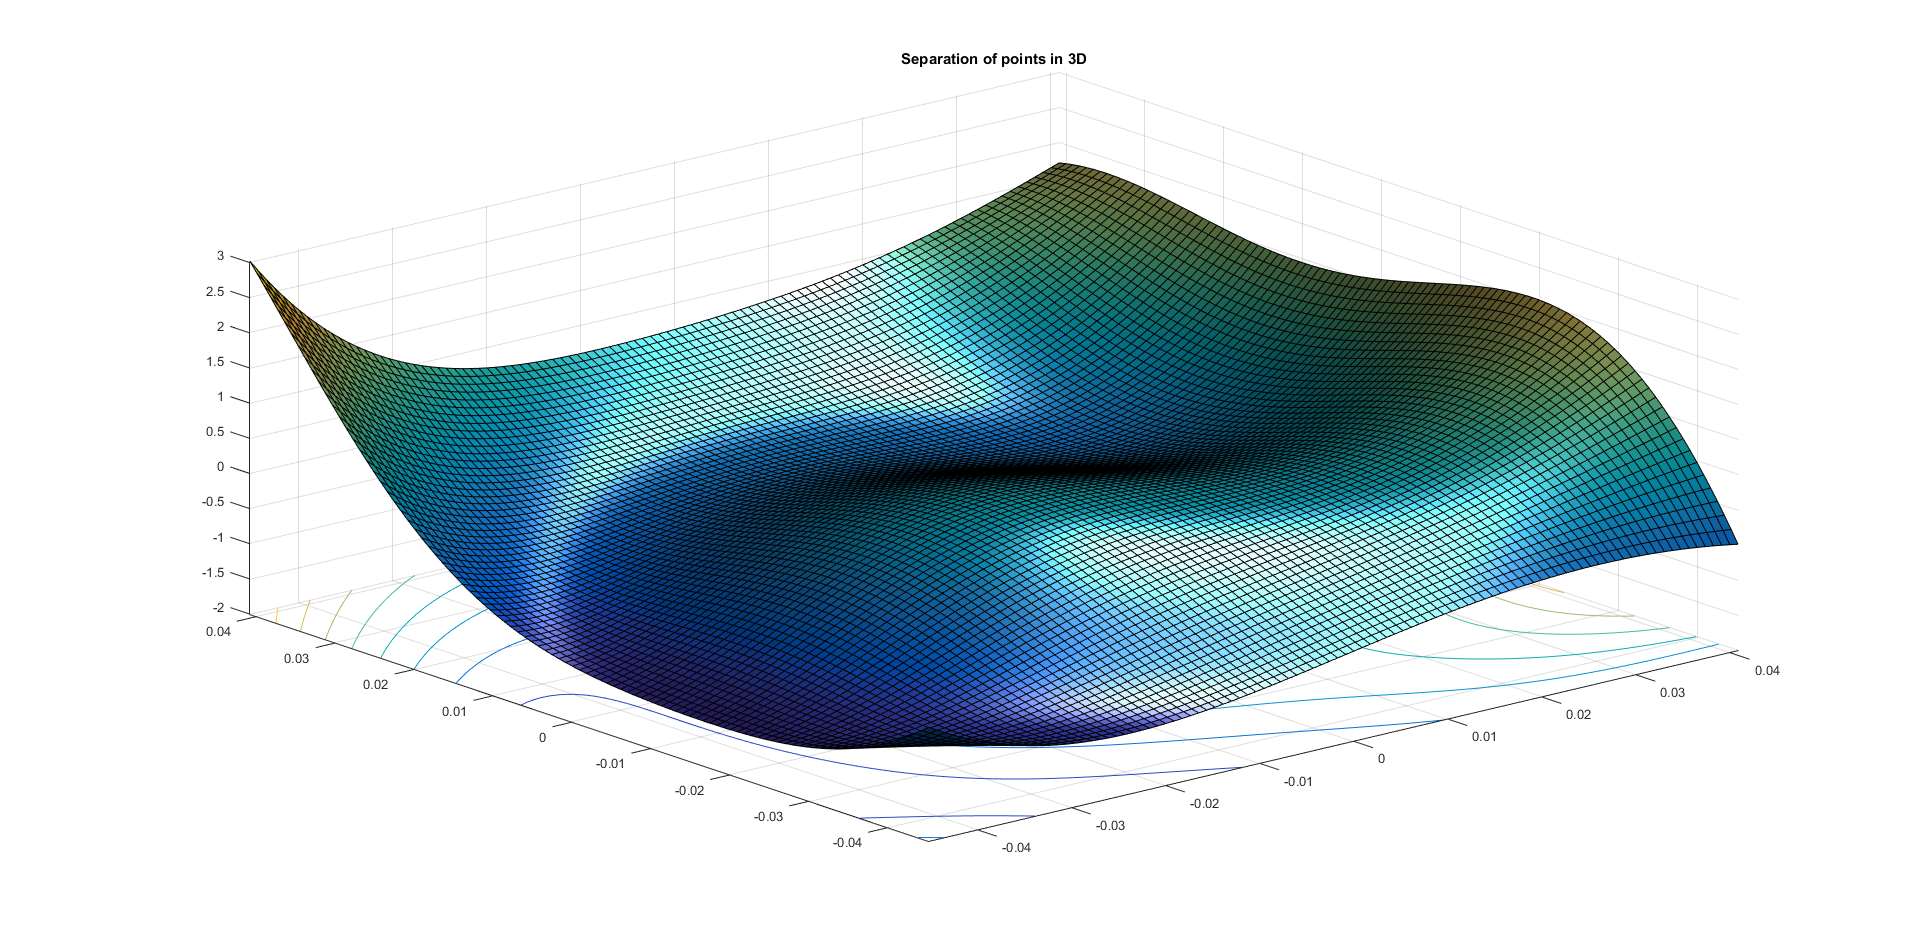
\includegraphics[width=0.242\textwidth]{figs/Contour_fibo_data.png}
  			\label{fig:contour_fibo}} 			
	\subfloat[Hyperplane Projection] 
	{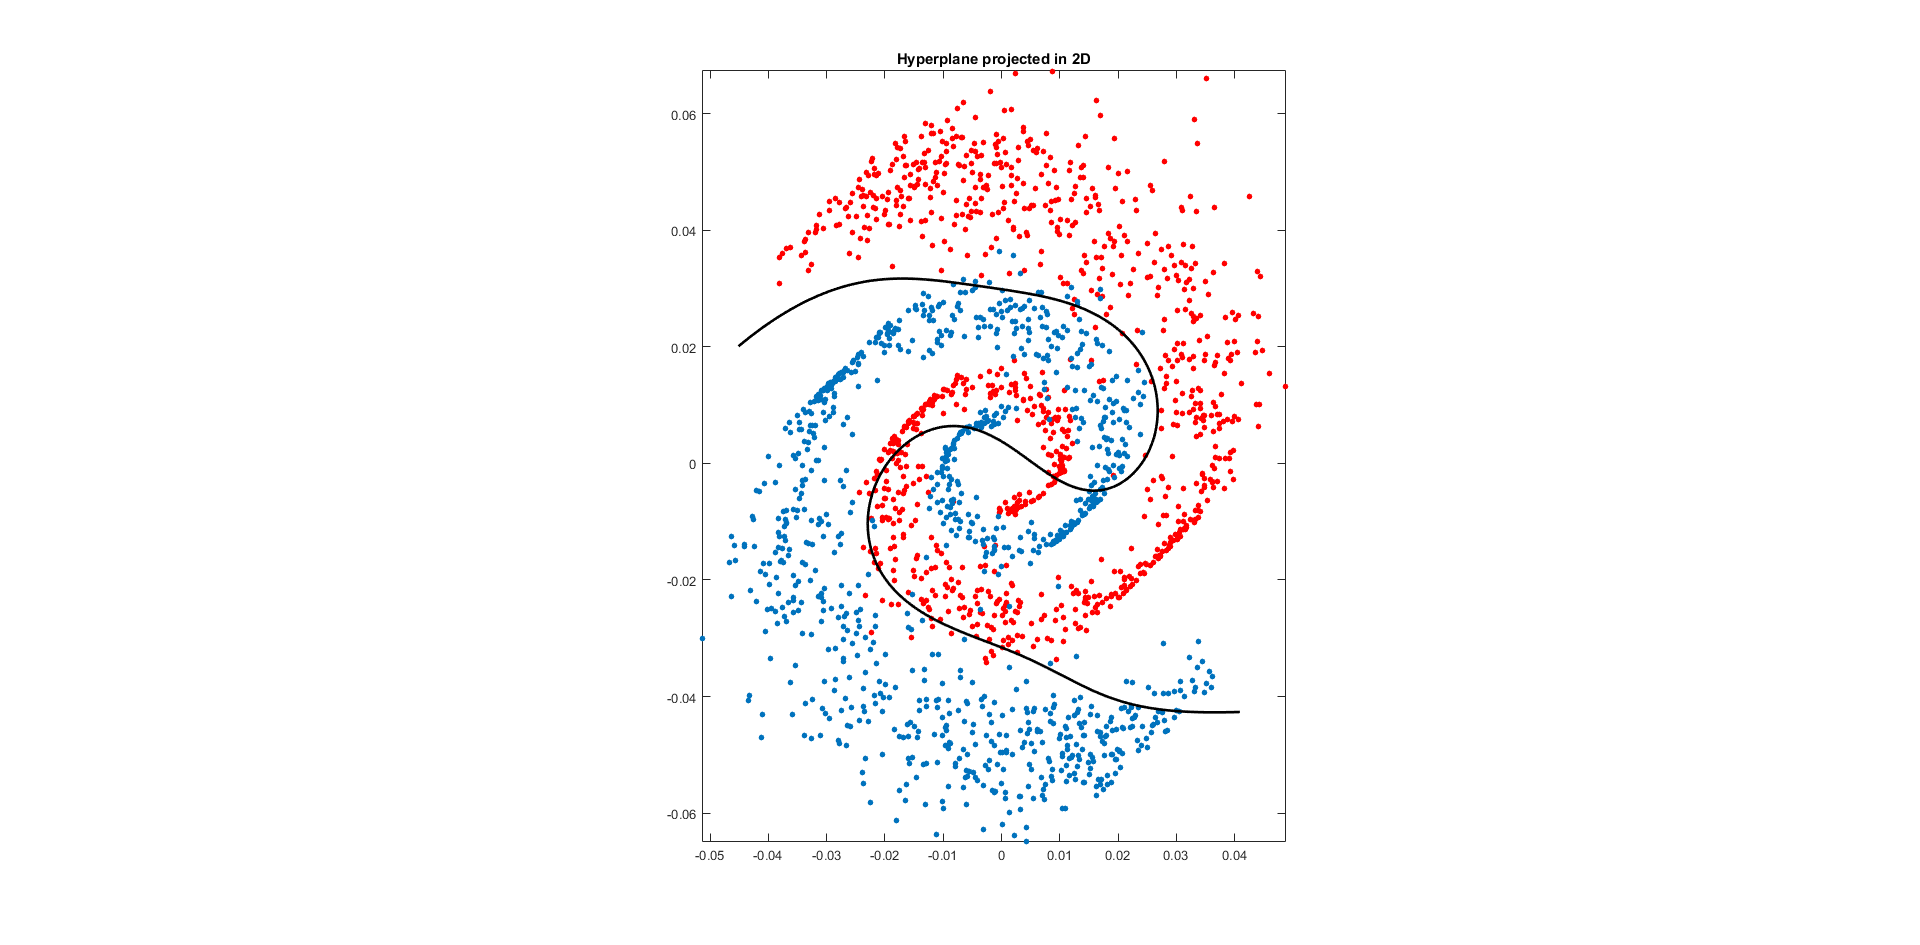
\includegraphics[width=0.242\textwidth]{figs/FB_spiral_HYP.png}
		\label{fig:fibo_spiral_hyp}} 
		\end{figure}
		
The only problem with the double spiral is the optimal separation of the blue and red points in every corner is going to take several iterations as the RBF kernel computes the dot products for the training model we setup earlier. Then we run the testing phase and see how unseen points are being separated by the hyperplane. The contours of the classifier is also plotted along with the error rate calculation.

Figure \ref{fig:perf} illustrates how varying different values of
sigma and cost changes the error rate. The gamma, sigma and the error rate value achieved for Fibonacci spiral are 0.0001, 0.043, 0.33 respectively. To illustrate what these values mean for actually separating the data, we show a plot of a good sigma, cost pair and a bad one. The dark blue values indicate a very low error rate. Choosing the optimal values of sigma and cost is another problem which is achieved after many iterations in MATLAB. The \textbf{RStudio} has different tuning options which help to optimize the SVM kernel we train and test samples
Lower values of sigma lead to over-fitting the data and choosing larger values might lead to separating the plane might not occur accurately.

\begin{figure}[bt!]
\centering
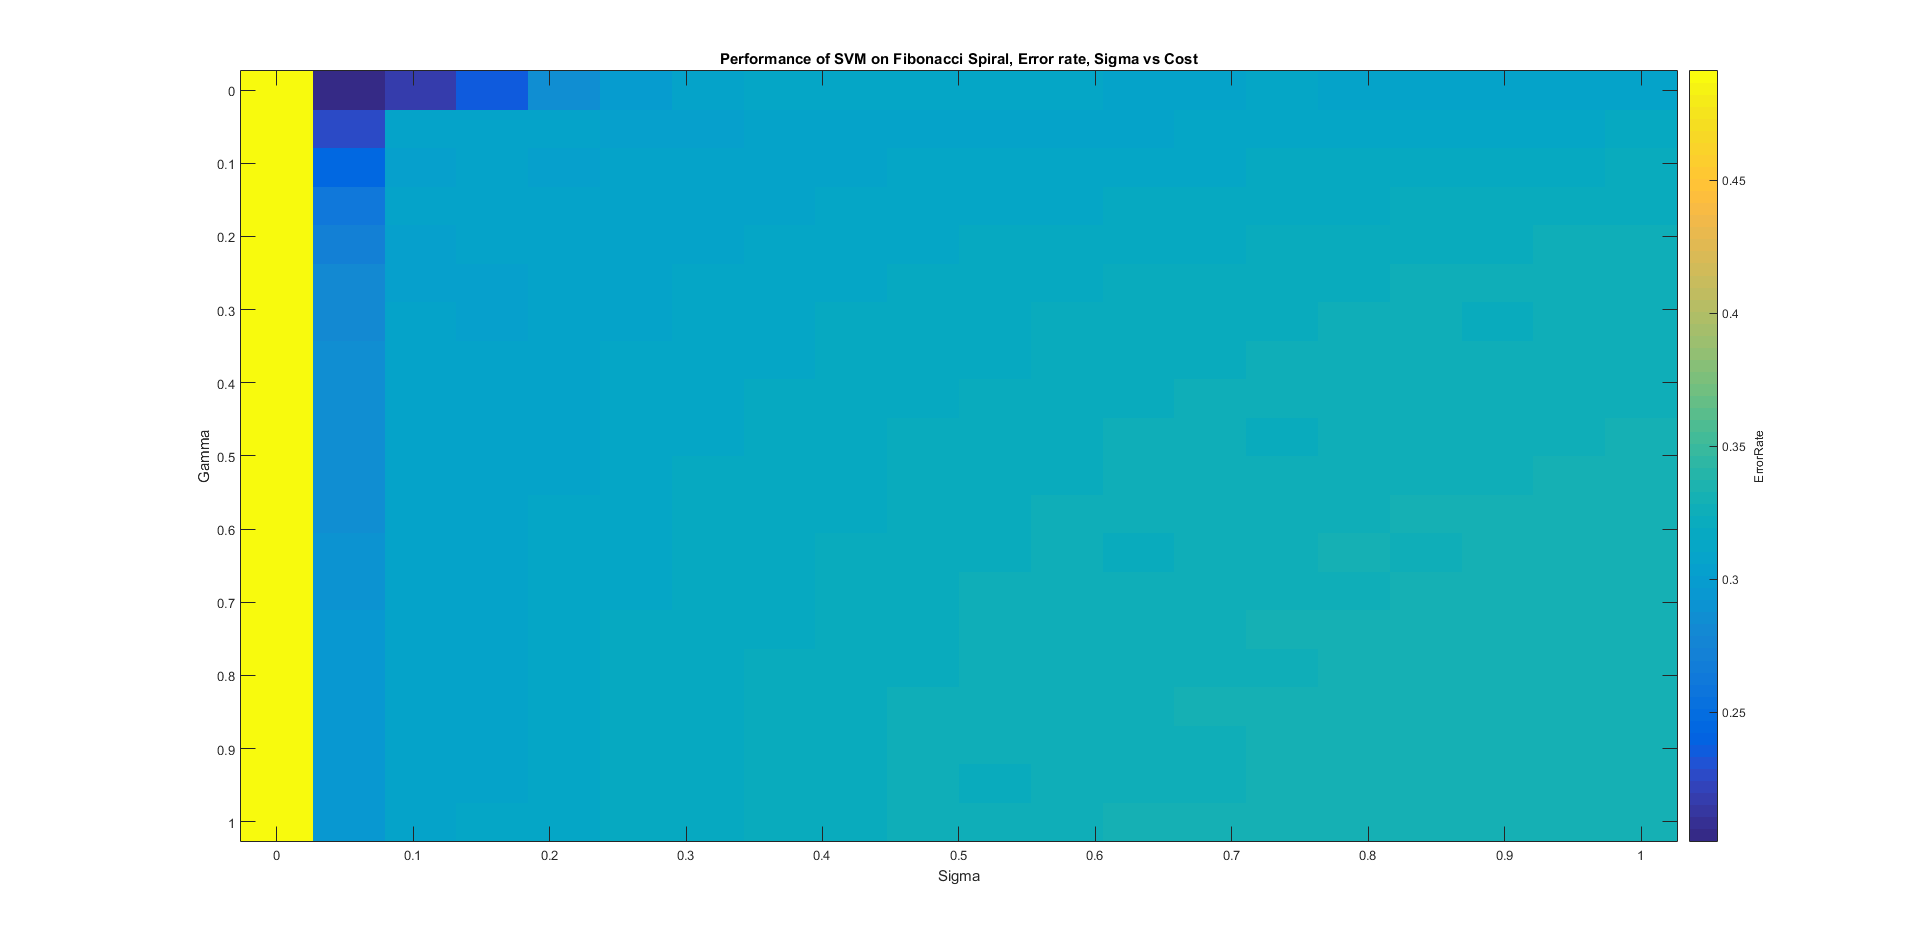
\includegraphics[width=0.5\textwidth]{figs/perf.png}
\caption{Error rates for different sigma cost combinations}
\label{fig:perf} 
\end{figure}

This proves that even thought we can have perfect training error, the testing
error can be much worse. This is due to a phenomenon called overfitting. In fact, 
you can choose a sigma and a cost such that you will always be able to get 
100\% training accuracy, but the model will not be good when faced with fitting
the testing data. 


\subsection{A Short History of Prognosis Breast Cancer UCI Dataset}
This work grew out of the desire by Dr. Wolberg to accurately diagnose breast masses based solely on a Fine Needle Aspiration (FNA). He identified nine visually assessed characteristics of an FNA sample which he considered relevant to diagnosis. In collaboration with Prof. Mangasarian and two of his graduate students, Rudy Setiono and Kristin Bennett, a classifier was constructed using the multisurface method (MSM) of pattern separation on these nine features that successfully diagnosed 97 of new cases. The resulting data set is well-known as the \textbf{ Wisconsin Breast Cancer Data}.

\subsection{SVM Classifier for Breast Cancer Dataset}
For the real-data I took the proposed challenge to setup SVM Classifiers for analyzing the Breast Cancer Wisconsin \cite{Mang1} \cite{Mang2} \cite{Mang1}(Prognostic) dataset \ref{table:Dataset} from UCI, Irvine that has a total number of data instances as 699 and the number of attributes are 10 plus the class attributes of which the the class distribution of tumors account to Benign 458 (65.5\%)  and Malignant 241 (34.5\%).

\begin{table}[h!]
	\center
	\caption{Wisconsin Breast Cancer Data Description}.
\label{table:Dataset}
\begin{tabular}{l|ll} 
		\hline
		\textbf{No.} & \textbf{Attributes} & \textbf{Domain} \\ 
		\hline 
		1.       &Sample code number  &ID number                 \\
		2.       &Clump Thickness     &1-10 \\
		3.       &Uniformity of Cell Size    & 1-10\\
		4.       &Uniformity of Cell Shape    & 1-10 \\
		5.       &Marginal Adhesion           &1-10 \\
		6.       &Single Epithelial Cell Size  & 1-10 \\
		7.       &Bare Nuclei                &1-10        \\
		8.       &Bland Chromatin             &1 - 10 \\
		9.       &Normal Nucleoli             &1-10 \\
		10.      &Mitoses                     &1-10      \\
		11.      &Class &(2 for benign, 4 for malignant)    \\
		\hline
	\end{tabular}
\end{table}


\subsubsection{SVM Classifier Experimental Setup}
For this setup, I used \textit{RStudio} ver \textbf{0.98} an integrated development environment (IDE) for R which works with the standard version of R available from CRAN. RStudio includes a wide range of packages that are extensively used in Statistics, Machine learning and Advanced Data Analysis etc. For SVM Classification, I used libSVM version of R known as library(e1071) and library(caret) for Classification and Regression modeling as standard package libraries. Then I split the dataset of 699 observations and after removing the missing attributes into training (456 points) and testing (227 points) sets with k-fold (10) cross-validation initially with a range of cost (c = 0.1,1,3,7,10) value and gamma(0.0001-0.1) for the SVM \ref{fig:svm_train}.

\begin{figure}[h]
\centering
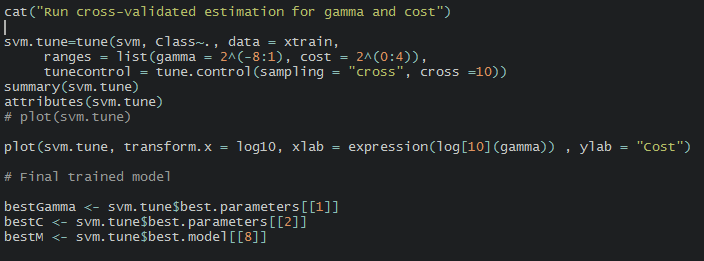
\includegraphics[width=3.3in]{figs/svm_train.png}
\caption{SVM model with initial training set 456}
\label{fig:svm_train} 
\end{figure}

From the SVM \cite{kernme}train model, we can obtain the best gamma, best Cost value and the best model by using the tuning function that does a grid search for the dual parameters, cost value and other attributes of the SVM. Then I use the SVM predict function for predicting the unseen or the testing data points and I have plotted the performance of SVM \ref{fig:perf95_svm} 

\begin{figure}[htb!]
\centering
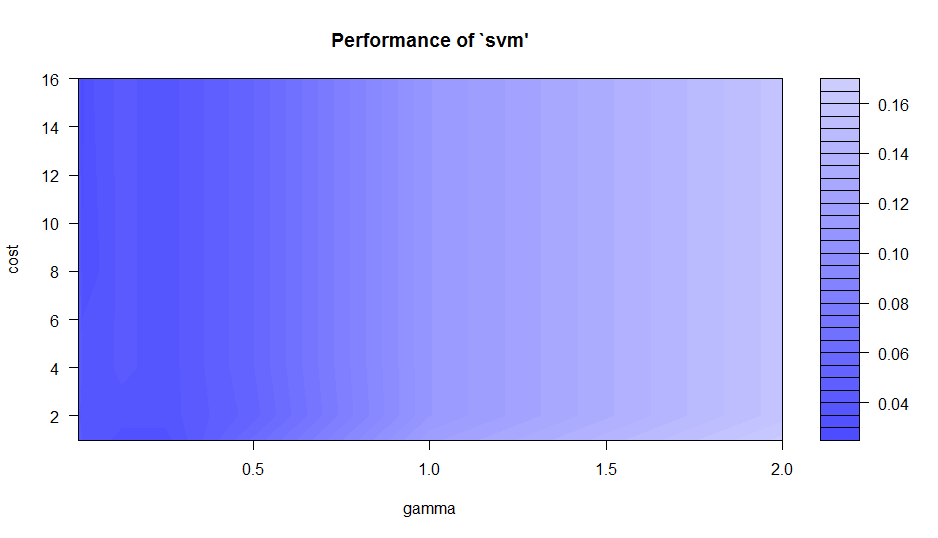
\includegraphics[width=3.25in]{figs/Perf95.png}
\caption{Performance of SVM after Tuning}
\label{fig:perf95_svm} 
\end{figure}
where the cost and the gamma values are together seen with dark blue values being the lowest cost value and error rate which will be discussed in the next results section .

\subsubsection{Results SVM Kernels}
I predicted the testing points using 1.Linear and 2.RBF  kernels and have plotted the confusion matrix and statistics for them given below.
\subsubsection{Linear Kernel}

\begin{figure}[h]
\centering
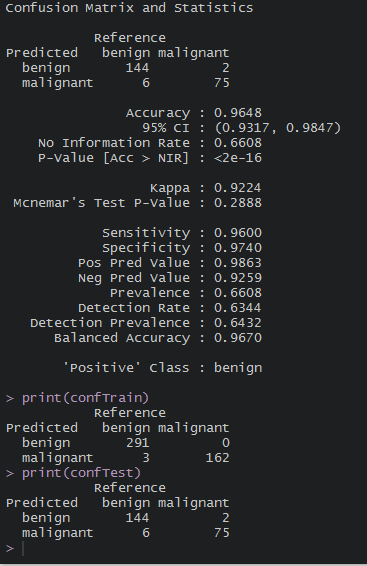
\includegraphics[width=0.5\textwidth]{figs/after_tuning_linear.png}
\caption{Confusion Matrix and Statistics for Linear Kernel}
\label{fig:LIN_ker} 
\end{figure}

Lets observe the confusion matrix of the linear \ref{fig:LIN_ker} kernel with benign tumors spotted correctly by 144 and malignant spotted at 75 with a few  misplaced classification. The accuracy is 96.48\% with sensitivity(0.96), specificity(0.97) and all class is positive Benign. Both the confusion matrices for training and testing sets are also computed here.
\subsubsection{RBF Kernel}

\begin{figure}[ht!]
\centering
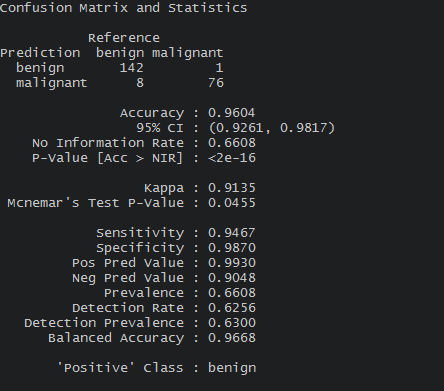
\includegraphics[width=0.5\textwidth]{figs/ConfMatRBF.png}
\caption{Confusion Matrix and Statistics for RBF Kernel}
\label{fig:RBF_conf} 
\end{figure}

In the confusion matrix \ref{fig:RBF_conf} of the RBF kernel \ref{fig:RBF_ker} we can see the Benign tumors \cite{UCI} are predicted at 142 and malignant 76 with few mis-classified labels. The accuracy is 96.04\% with sensitivity(0.94), specificity(0.98) and all class is positive Benign. Also the best model after tuning of the SVM with RBF kernel has a sigma value(0.018) and cost(0.5) significantly reducing the complexity and the computation of the gamma,sigma and cost calculations since we tuned the SVM to find the optimally best values to be used for prediction of new points.

\begin{figure}[ht!]
\centering
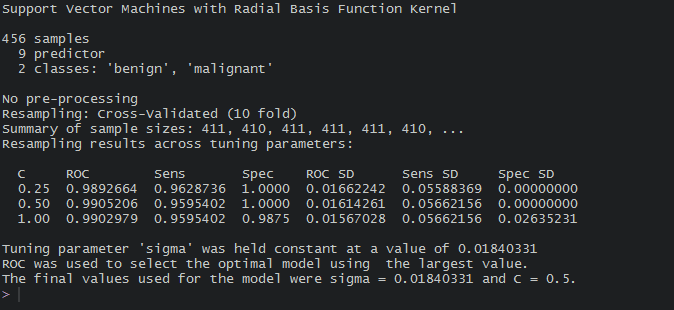
\includegraphics[width=0.6\textwidth]{figs/after_tuning_radial.png}
\caption{Tuning results for RBF Kernel}
\label{fig:RBF_ker} 
\end{figure}

\section{Results Comparison}

Past Usage: Attributes 2 through 10 have been used to represent instances. Each instance has one of 2 possible classes: benign or malignant.

\subsection*{Wolberg Group} 
\begin{table}[h!]
\center
	\caption{Wolberg Results 1990}
\label{table:Wol_Results} \cite{wolberg}

   1. Wolberg,W.H., \& Mangasarian,O.L. (1990). Multisurface method of 
      pattern separation for medical diagnosis applied to breast cytology. In
      {\textit Proceedings of the National Academy of Sciences}, {\textit 87},
      9193--9196.
      -- Size of data set: only 369 instances (at that point in time)
      -- Collected classification results: 1 trial only
      -- Two pairs of parallel hyperplanes were found to be consistent with
         50\% of the data
         -- Accuracy on remaining 50\% of dataset: 93.5\%
      -- Three pairs of parallel hyperplanes were found to be consistent with
         67\% of data
         -- Accuracy on remaining 33\% of dataset: 95.9\%
\end{table}



\subsection*{Zhang Group}
\begin{table}[h!]
\center
	\caption{Zhang Results 1992}
\label{table:Zhang_Results} \cite{zhang}

	Zhang,J. (1992). Selecting typical instances in instance-based
      learning.  In {\textit{ Proceedings of the Ninth International Machine
      Learning Conference}} (pp. 470--479).  Aberdeen, Scotland: Morgan
      Kaufmann.
      -- Size of data set: only 369 instances (at that point in time)
      -- Applied 4 instance-based learning algorithms 
      -- Collected classification results averaged over 10 trials
      -- Best accuracy result: 
         -- 1-nearest neighbor: 93.7\%
         -- trained on 200 instances, tested on the other 169
      -- Also of interest:
         -- Using only typical instances: 92.2\% (storing only 23.1 instances)
         -- trained on 200 instances, tested on the other 169
\end{table}

\subsection*{UNM 2015 Machine Learning Class results}
\begin{table}[h!]
\center
	\caption{UNM 2015 Machine Learning Class results}
\label{table:My_Results}
 Compared with the past usage of this dataset.
	  -- Size of data set: only 699 instances (at that point in time)
      -- Applied 10 Cross-validation based learning SVM kernels.
      -- Collected classification results averaged over 10 trials
      -- Best accuracy result: 
         -- SVM RBF Kernel: 96.8\%
         -- SVM Linear Kernel: 96.4\%
         -- trained on 456 instances, tested on the other 227
\end{table}

\section{Conclusion}
In this paper, we have studied the kernels from simple XOR problem to Double Fibonacci spiral to understand the working of kernels in Hilbert space dimensions.Using that, we have appropriately used SVM kernels to study and analyze an real-world dataset. The real-world experiment is done after careful observation of the training data and cross-validated to accurately predict the new data which can be used to test on new data from this dataset. Further research on kernels have helped to understand the working of SVM kernels.
%
%\bibliographystyle{IEEEbib}{1}
%\bibliography{HW2}

\begin{thebibliography}{1}

\bibitem{wolberg}
Wolberg,W.H., \& Mangasarian,O.L. (1990). Multisurface method of 
      pattern separation for medical diagnosis applied to breast cytology. In
      {\textit Proceedings of the National Academy of Sciences}, {\textit 87},
      9193--9196

\bibitem{zhang}
Zhang,J. (1992). Selecting typical instances in instance-based
      learning.  In {\textit{ Proceedings of the Ninth International Machine
      Learning Conference}} (pp. 470--479).  Aberdeen, Scotland: Morgan
      Kaufmann

\bibitem{UCI}
UCI Machine Learning Repository: Breast Cancer Wisconsin (Diagnostic) Data Set (January 2011) by William H. Wolberg, W. Nick Street, Olvi L. Mangasarian

\bibitem{Mang1}
Mangasarian and W. H. Wolberg: "Cancer diagnosis via linear 
      programming", SIAM News, Volume 23, Number 5, September 1990, pp 1 \& 18.

\bibitem{Mang2}
O. L. Mangasarian, R. Setiono, and W.H. Wolberg: "Pattern recognition 
      via linear programming: Theory and application to medical diagnosis", 
      in: "Large-scale numerical optimization", Thomas F. Coleman and Yuying
      Li, editors, SIAM Publications, Philadelphia 1990, pp 22-30.

\bibitem{KPB}
K. P. Bennett \& O. L. Mangasarian: "Robust linear programming 
      discrimination of two linearly inseparable sets", Optimization Methods
      and Software 1, 1992, 23-34 (Gordon \& Breach Science Publishers).
      
\bibitem{kernme},
Cristianini, Nello, Shawe-Taylor, John, "Kernel Methods for Pattern Analysis",
Cambridge University Press, 2004.


\end{thebibliography}

\end{document}  
%